%================================================
% TASK 1.1
%================================================
\section{Task 1.1: Sliding Window -- Most Bought Size per State}

\subsection{Phân tích truy vấn}
Bài toán yêu cầu xác định kích cỡ được mua nhiều nhất tại từng bang/tỉnh theo từng ngày tính toán $d$. Với mỗi ngày $d$, cửa sổ thời gian chỉ xét tối đa 7 ngày trước đó, tức $[d-7, d-1]$, không bao gồm ngày hiện tại. Vì cửa sổ trượt từng ngày nên kết quả đầu ra có thể chứa các ngày không có đơn hàng trực tiếp trong dữ liệu gốc, kể cả các ngày ngay sau ngày đơn hàng cuối cùng nếu cửa sổ quá khứ vẫn còn dữ liệu đóng góp.

Một dòng dữ liệu được xem là ``được mua'' khi thỏa đồng thời hai điều kiện: cột \texttt{Status} chứa chuỗi \texttt{shipped} sau khi chuẩn hóa chữ hoa/thường, và cột \texttt{Qty} là số nguyên dương. Cách hiểu này bao phủ các trạng thái như \texttt{Shipped}, \texttt{Shipped - Delivered to Buyer}, \texttt{Shipped - Returned to Seller}, đúng với mô tả trong đề bài là trạng thái đơn hàng có chứa ``shipped''.

Đơn vị đo ``mua nhiều nhất'' trong lời giải là tổng số lượng (\texttt{Qty}) theo kích cỡ trong cửa sổ, không chỉ đơn thuần là số dòng đơn hàng. Với mỗi khóa \texttt{(ship-state, date)}, chương trình so sánh tổng số lượng của từng kích cỡ và chọn kích cỡ có tổng lớn nhất. Nếu nhiều kích cỡ có cùng tổng số lượng, chương trình phá hòa bằng thứ tự từ điển tăng dần của chuỗi kích cỡ để kết quả ổn định và tái lập được.

Kết quả đầu ra của nhiệm vụ này là một tệp CSV thông thường trên hệ thống tệp, có dòng đầu chứa tiêu đề và đúng tên \texttt{Task\_1-1.csv}. Cấu trúc dữ liệu thực tế:

\begin{table}[H]
\centering
\begin{tabular}{lll}
\toprule
\textbf{Cột} & \textbf{Kiểu dữ liệu} & \textbf{Ý nghĩa} \\
\midrule
\texttt{ship-state} & String & Bang/tỉnh cần tính toán \\
\texttt{date} & String & Ngày tính toán $d$, định dạng \texttt{MM-dd-yy} \\
\texttt{most\_bought\_size} & String & Kích cỡ có tổng số lượng cao nhất trong cửa sổ \\
\texttt{max\_quantity} & Integer & Tổng số lượng của kích cỡ thắng cuộc trong cửa sổ \\
\bottomrule
\end{tabular}
\caption{Định nghĩa schema tệp đầu ra Task\_1-1.csv}
\label{tab:task1_1_schema}
\end{table}

\subsection{Phân rã thành các bước cơ bản}
Lời giải được triển khai theo tư duy MapReduce trên Spark RDD, gồm các bước sau:

\begin{enumerate}
    \item \textbf{Đọc và kiểm tra cấu trúc dữ liệu đầu vào.} Chương trình đọc tệp CSV, phân tích dòng đầu và kiểm tra đủ các cột bắt buộc: \texttt{Date}, \texttt{Status}, \texttt{Qty}, \texttt{Size}, \texttt{ship-state}. Nếu thiếu cột, chương trình dừng với thông báo lỗi rõ ràng.
    \item \textbf{Phân tích và chuẩn hóa bản ghi.} Mỗi dòng được phân tích cú pháp bằng bộ phân tích CSV tự viết để xử lý dấu phẩy nằm trong các trường có dấu nháy kép. Ngày được phân tích theo các định dạng phổ biến như \texttt{MM-dd-yy}, \texttt{M-d-yy}, \texttt{MM/dd/yy}, \texttt{M/d/yy}; cột \texttt{Qty} được chuyển kiểu sang số nguyên dương; cột \texttt{ship-state} được loại bỏ khoảng trắng thừa (\texttt{trim}) và chuẩn hóa viết hoa để tránh tách cùng một bang thành nhiều khóa khác nhau.
    \item \textbf{Lọc các mặt hàng được mua thực tế.} Chỉ giữ các dòng có trạng thái \texttt{Status} chứa từ khóa \texttt{shipped}, số lượng \texttt{Qty > 0}, đồng thời tên bang \texttt{ship-state} và kích cỡ \texttt{Size} không bị rỗng. Bước này giúp giảm lượng dữ liệu trung gian trước khi phát sinh các khóa cửa sổ.
    \item \textbf{Sinh đóng góp cho cửa sổ trượt.} Với mỗi giao dịch mua hợp lệ tại ngày $t$, chương trình phát ra đóng góp cho các ngày tính toán trong tương lai $d = t+1, t+2, \ldots, t+7$. Điều này tương đương với việc giao dịch tại ngày $t$ nằm trong cửa sổ quá khứ của các ngày tính toán $d$ đó.
    \item \textbf{Cộng tổng số lượng theo khóa \texttt{(state, day, size)}.} Các đóng góp cùng bang, cùng ngày tính toán và cùng kích cỡ được cộng dồn bằng phép biến đổi \texttt{reduceByKey}.
    \item \textbf{Chọn kích cỡ thắng cuộc theo khóa \texttt{(state, day)}.} Kết quả ở bước trước được đổi khóa thành \texttt{(state, day)}, sau đó bộ giảm chọn kích cỡ có tổng số lượng lớn nhất; nếu xảy ra hòa thì chọn kích cỡ có thứ tự từ điển nhỏ hơn.
    \item \textbf{Sắp xếp và ghi ra tệp CSV duy nhất.} Kết quả được sắp xếp theo bang \texttt{state} và ngày \texttt{day}, thêm dòng tiêu đề, dùng \texttt{coalesce(1)} để ghi ra một thư mục tạm, sau đó đổi tên tệp bộ phận thành tệp CSV duy nhất có tên chính xác theo yêu cầu.
\end{enumerate}

\subsection{Lý do phân rã}
Phần khó nhất của bài toán là cơ chế cửa sổ trượt. Nếu tính trực tiếp cho từng ngày $d$ rồi quét ngược lại 7 ngày trước đó, chi phí quét dữ liệu sẽ lặp lại nhiều lần. Lời giải chọn hướng tiếp cận ngược lại: một đơn hàng tại ngày $t$ tự phát sinh đóng góp cho tối đa 7 ngày tương lai mà nó có thể thuộc về cửa sổ. Nhờ vậy, cửa sổ trượt được chuyển đổi thành bài toán gom nhóm khóa - giá trị thông thường.

Cách phân rã này hoàn toàn phù hợp với MapReduce vì mỗi bước đều có khóa rõ ràng. Bước ánh xạ sinh khóa \texttt{(state, day, size)}; bước giảm đầu tiên cộng số lượng; bước reduce thứ hai chọn kích cỡ thắng cuộc cho từng khóa \texttt{(state, day)}. Việc lọc dữ liệu hợp lệ trước khi phát sinh 7 đóng góp cũng giúp giảm thiểu số lượng bản ghi trung gian và giảm chi phí truyền tải dữ liệu qua mạng.

\subsection{Chiến lược thực thi \& Triển khai mã nguồn}
Task 1.1 được cài đặt trong file \texttt{src/Task\_1-1/source/Task1\_1.scala}. Chương trình nhận hai tham số: đường dẫn CSV đầu vào và đường dẫn file CSV đầu ra. Logic chính dùng Spark RDD transformations như \texttt{mapPartitions}, \texttt{flatMap}, \texttt{reduceByKey}, \texttt{sortBy}, \texttt{saveAsTextFile}; không dùng DataFrame query hoặc Spark SQL cho phần tính toán.

\textbf{Lệnh chạy mẫu:}
\begin{lstlisting}[language=bash]
cat > /tmp/task1_1.runner.scala <<'EOF'
:load src/Task_1-1/source/Task1_1.scala
Task1_1.main(Array("data/input/Amazon Sale Report.csv",
  "data/output/Task_1-1.csv"))
sys.exit(0)
EOF
SPARK_LOCAL_IP=127.0.0.1 SPARK_LOCAL_HOSTNAME=localhost \
  spark-shell < /tmp/task1_1.runner.scala
\end{lstlisting}

\textbf{Parse và lọc purchase hợp lệ.}
\begin{lstlisting}[language=Scala]
val purchases = parsedRows.flatMap { case (epochDay, state, size, status, qtyText) =>
  parsePositiveInt(qtyText).filter(_ => status.contains("shipped")).flatMap { qty =>
    if (state.nonEmpty && size.nonEmpty) Some(Purchase(epochDay, state, size, qty))
    else None
  }
}
\end{lstlisting}

\textbf{Sinh đóng góp cho sliding window.}
\begin{lstlisting}[language=Scala]
val windowContributions = purchases.flatMap { purchase =>
  (1L to 7L).iterator.flatMap { offset =>
    val targetDay = purchase.orderEpochDay + offset
    if (targetDay >= minEpochDay) {
      Some(((purchase.state, targetDay, purchase.size), purchase.qty))
    } else {
      None
    }
  }
}
\end{lstlisting}

\textbf{Cộng tổng quantity và chọn size thắng.}
\begin{lstlisting}[language=Scala]
val sizeTotals = windowContributions.reduceByKey(_ + _)

val winners = sizeTotals
  .map { case ((state, day, size), totalQty) => ((state, day), (size, totalQty)) }
  .reduceByKey { (left, right) =>
    val (leftSize, leftQty) = left
    val (rightSize, rightQty) = right
    if (leftQty > rightQty) left
    else if (rightQty > leftQty) right
    else if (leftSize <= rightSize) left
    else right
  }
\end{lstlisting}

\subsection{Phân tích chuyên sâu}

\subsubsection{Pseudocode tổng quan}

\begin{algorithm}[H]
\caption{Sliding Window --- Most Bought Size per State (MapReduce)}
\label{alg:task1_1}
\begin{algorithmic}[1]
\Require Dataset $\mathcal{D}$ with columns (Date, Status, Qty, Size, ship-state)
\Ensure CSV file: (State, Date $d$, MostBoughtSize, MaxQty)
\Statex
\State $d_{\min} \gets$ min epoch day in $\mathcal{D}$
\Statex
\Statex \textbf{--- MAP PHASE ---}
\ForAll{row $r \in \mathcal{D}$ where Status contains ``shipped'' $\wedge$ Qty $> 0$}
    \State $t \gets$ epochDay(r.Date)
    \For{$\delta = 1$ \textbf{to} $7$}
        \If{$d_{\min} \leq t + \delta$}
            \State \textbf{emit} $\langle$(r.State, $t + \delta$, r.Size), r.Qty$\rangle$
        \EndIf
    \EndFor
\EndFor
\Statex
\Statex \textbf{--- REDUCE PHASE 1 ---}
\ForAll{key (State, Day, Size)}
    \State totalQty $\gets \sum$ values \Comment{reduceByKey(\_ + \_)}
\EndFor
\Statex
\Statex \textbf{--- REDUCE PHASE 2 ---}
\ForAll{key (State, Day)}
    \State winner $\gets \arg\max_{\text{Size}}$ totalQty \Comment{tie-break: lexicographic}
    \State \textbf{emit} (State, Day, winner.Size, winner.Qty)
\EndFor
\end{algorithmic}
\end{algorithm}

Phạm vi cửa sổ trượt cho ngày tính toán $d$ được định nghĩa:
\[
W(d) = [d - 7,\; d - 1]
\]
Tương đương, một giao dịch tại ngày $t$ đóng góp cho các ngày tính toán $d \in [t+1,\; t+7]$.

\subsubsection{Tại sao vòng lặp lồng nhau ngây thơ bất khả thi}

Cách tiếp cận trực tiếp là: với mỗi ngày tính toán $d$ và mỗi bang $s$, quét toàn bộ bộ dữ liệu để lọc các dòng có ngày thuộc khoảng $[d-7, d-1]$ và cùng bang, rồi đếm số lượng theo kích cỡ. Gọi $D$ là số ngày khác nhau, $S$ là số bang, $N$ là tổng số dòng dữ liệu; phương pháp này có chi phí thời gian lên tới $O(D \times S \times N)$. Với $D \approx 120$, $S \approx 36$, $N \approx 128\,000$, số phép so sánh cần thực hiện là $\sim 5.5 \times 10^8$ --- quá tốn kém và hoàn toàn không tận dụng được kiến trúc tính toán song song của mô hình MapReduce.

\subsubsection{Thiết kế khóa giải quyết vấn đề thế nào}

Thay vì quét ngược từ ngày tính toán $d$ về quá khứ, lời giải áp dụng cơ chế ``đẩy xuôi'' từ phía giao dịch: một đơn hàng xảy ra tại ngày $t$ sẽ tự động phát sinh ra tối đa 7 bản ghi đóng góp cho các ngày tính toán tương lai từ $t+1$ đến $t+7$. Khóa được phát ra là \texttt{(state, targetDay, size)}, chuyển đổi cơ chế cửa sổ trượt thành bài toán gom nhóm khóa - giá trị thông thường:

\begin{itemize}
    \item \textbf{Bước giảm lần 1} (\texttt{reduceByKey}): Cộng tổng số lượng cho mỗi khóa \texttt{(state, day, size)}. Chi phí: mỗi giao dịch phát sinh tối đa 7 đóng góp ($O(7N)$ bản ghi trung gian), sau đó tiến hành phân tán và cộng dồn song song.
    \item \textbf{Bước giảm lần 2}: Đổi khóa thành \texttt{(state, day)} để gom toàn bộ các kích cỡ cùng bang và ngày tính toán, từ đó chọn ra kích cỡ có tổng số lượng lớn nhất. Nếu xảy ra hòa, phá hòa bằng thứ tự từ điển tăng dần của chuỗi kích cỡ.
\end{itemize}

Phương pháp này chỉ tốn chi phí $O(7N)$ cho bước ánh xạ và $O(K \log K)$ cho bước sắp xếp và giảm (với $K$ là số lượng khóa khác nhau), hiệu quả hơn nhiều bậc so với cách tiếp cận ngây thơ.

\subsubsection{Xử lý các ngày trống không có giao dịch}

Ví dụ: nếu không có đơn hàng nào xảy ra vào ngày 04-05-22 nhưng có các đơn hàng trong khoảng từ 03-29-22 đến 04-04-22, ngày 04-05-22 vẫn phải xuất hiện trong kết quả đầu ra vì cửa sổ $[03-29, 04-04]$ của nó có dữ liệu đóng góp.

Cơ chế phát đóng góp tự động giải quyết vấn đề này: giao dịch mua tại ngày $t$ khi phát đóng góp cho $t+1$ đến $t+7$ sẽ tự động điền dữ liệu vào các ngày trống này. Đồng thời, đối với các đơn hàng cuối cùng (ví dụ ngày 06-29-22), cửa sổ trượt cho phép kết quả kéo dài đến ngày 07-06-22 do các giao dịch cuối này vẫn nằm trong cửa sổ quá khứ của những ngày tiếp sau.

\subsection{Kết quả thực thi \& Xuất dữ liệu}
Tệp kết quả đầu ra đã được tạo tại \texttt{data/output/Task\_1-1.csv}. Tệp có 3,544 dòng bao gồm dòng tiêu đề, tương ứng 3,543 dòng kết quả. Một số dòng đầu của kết quả:

\begin{lstlisting}[language={}]
ship-state,date,most_bought_size,max_quantity
ANDAMAN & NICOBAR,04-02-22,M,1
ANDAMAN & NICOBAR,04-03-22,S,2
ANDAMAN & NICOBAR,04-04-22,S,3
ANDAMAN & NICOBAR,04-05-22,S,3
ANDAMAN & NICOBAR,04-06-22,S,3
ANDAMAN & NICOBAR,04-07-22,S,4
ANDAMAN & NICOBAR,04-08-22,S,4
ANDAMAN & NICOBAR,04-09-22,XL,5
\end{lstlisting}

\textbf{Kiểm chứng thủ công.} Với bang \texttt{ANDAMAN \& NICOBAR} và ngày tính toán \texttt{04-09-22}, cửa sổ quá khứ được xác định từ ngày \texttt{04-02-22} đến hết ngày \texttt{04-08-22}. Sau khi lọc các đơn hàng hợp lệ (Status chứa \texttt{shipped} và số lượng \texttt{Qty > 0}), tổng số lượng theo kích cỡ trong cửa sổ quá khứ này là:

\begin{table}[H]
\centering
\begin{tabular}{lr}
\toprule
\textbf{Size} & \textbf{Tổng Qty trong window} \\
\midrule
XL & 5 \\
L & 4 \\
S & 4 \\
XS & 4 \\
XXL & 3 \\
3XL & 1 \\
M & 1 \\
\bottomrule
\end{tabular}
\caption{Thống kê tổng số lượng (Qty) theo kích cỡ trong cửa sổ quá khứ tại bang Andaman \& Nicobar vào ngày 04-09-22}
\label{tab:task1_1_manual_check}
\end{table}

Kích cỡ \texttt{XL} có tổng số lượng cao nhất là 5, khớp hoàn toàn với dòng kết quả đầu ra \texttt{ANDAMAN \& NICOBAR,04-09-22,XL,5}. Phép kiểm chứng này xác nhận cơ chế phát đóng góp hoạt động hoàn toàn chính xác.

\subsection{Minh chứng bằng hình ảnh}
Các hình dưới đây là minh chứng chạy chương trình, xem trước kết quả đầu ra và kiểm chứng thủ công cho Task 1.1.

\begin{figure}[H]
    \centering
    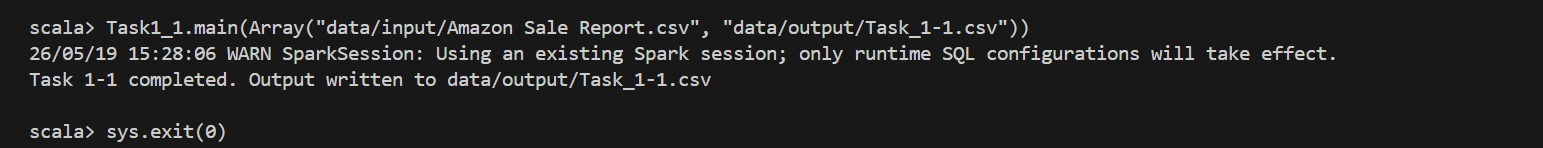
\includegraphics[width=0.9\textwidth]{img/1-1/run_success.png}
    \caption{Kết quả chạy chương trình Task 1.1}
    \label{fig:task1_1_run_success}
\end{figure}

\begin{figure}[H]
    \centering
    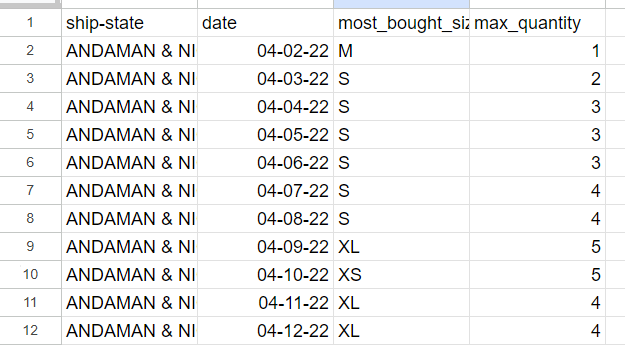
\includegraphics[width=0.9\textwidth]{img/1-1/output_preview.png}
    \caption{Một phần nội dung file \texttt{Task\_1-1.csv}}
    \label{fig:task1_1_output_preview}
\end{figure}

\begin{figure}[H]
    \centering
    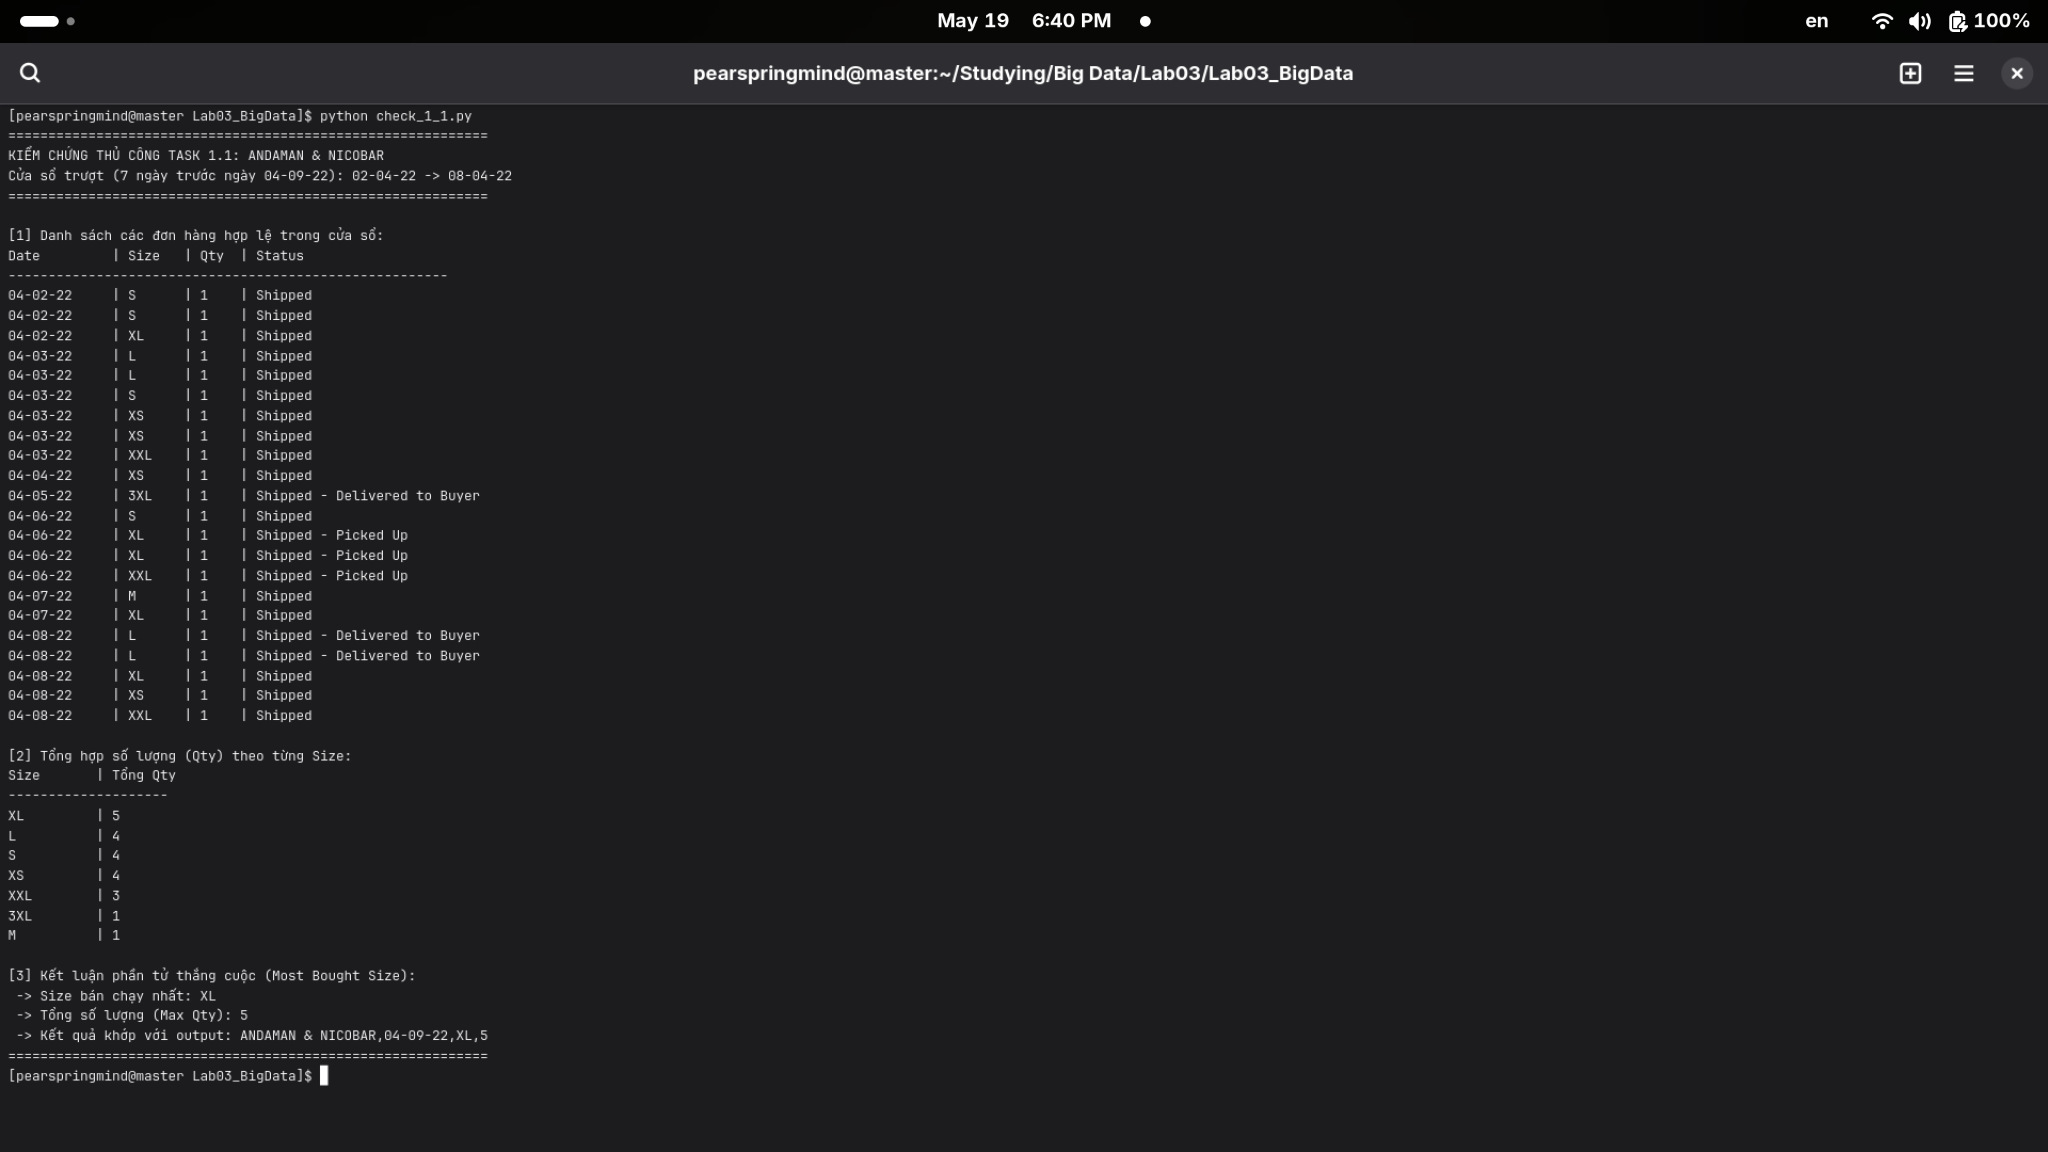
\includegraphics[width=0.9\textwidth]{img/1-1/manual_check.png}
    \caption{Kiểm chứng thủ công sliding window cho một state-date mẫu}
    \label{fig:task1_1_manual_check}
\end{figure}
